\documentclass[a4paper,12pt]{scrartcl}
\usepackage[ngerman]{babel}
\usepackage[T1]{fontenc}
\usepackage{lmodern}
\usepackage{blindtext}
\usepackage{tabularx}
\usepackage[utf8]{inputenc}
\usepackage{amsmath}
\usepackage{tikz}
\usetikzlibrary{arrows,shapes,positioning,shadows,trees}
\usepackage{forest}
\usetikzlibrary{shadows,arrows.meta}
\usepackage{rotating}
\usepackage{geometry}
\usepackage{graphicx}
\usepackage{acronym}
\usepackage{amsfonts}
\usepackage{hhline,booktabs}
\usepackage{siunitx}
\usepackage{amssymb}% http://ctan.org/pkg/amssymb
\usepackage{pifont}% http://ctan.org/pkg/pifont
\usepackage{textcomp}
\usepackage{eurosym}
\usepackage{forest}
\usepackage{tikz-qtree}
\usetikzlibrary{arrows.meta, shapes.geometric, calc, shadows}
\usepackage{booktabs}
\usepackage{dcolumn}
\makeatletter
\newcolumntype{d}[1]{>{\DC@{,}{,}{#1}}l<{\DC@end}}
\makeatother
\usetikzlibrary{positioning}
\usepackage{mathtools, nccmath}
\usepackage{adjustbox}
\usepackage{pgfgantt}
\usetikzlibrary{calc} 
\usetikzlibrary{arrows.meta} 
\usetikzlibrary{positioning}
\usepackage{verbatim}
\usetikzlibrary{arrows.meta}
\usepackage{booktabs}
\usepackage{xcolor}
\usepackage{colortbl}
\usepackage{longtable}
\usepackage{ulem}
\usepackage{amsthm}
\usepackage{ulem}
\usepackage{setspace}
\usepackage{float}

%\bibliographystyle{unsrt}
%\addbibresource{LiteraturIntelligenteSensoren}
%Zitationsstil
\usepackage{cite}
%cite{...} -> Drag and Drop von Citavi

%gantt
\newganttchartelement*{rresource}{
    rresource/.style={},
    inline=true,
    rresource inline label node/.style={anchor=west,font=\bfseries\itshape\color{blue}},
    rresource left shift=0ex,
    rresource right shift=0ex
}
\newganttchartelement*{lresource}{ % The starred version mimics a milestone element with 2 options
    lresource/.style={}, % Don't draw the node
    inline=true,
    lresource inline label node/.style={anchor=east,font=\bfseries\itshape\color{blue}},
    lresource left shift=0ex,
    lresource right shift=0ex
}
%gantt
\makeatletter
\newcommand{\ccell}[3][]{%
  \kern-\fboxsep
  \if\relax\detokenize{#1}\relax
    \expandafter\@firstoftwo
  \else
    \expandafter\@secondoftwo
  \fi
  {\colorbox{#2}}%
  {\colorbox[#1]{#2}}%
  {#3}\kern-\fboxsep
}
\makeatother
\definecolor{cellgray}{gray}{0.9}
\definecolor{pastelred}{rgb}{1.0, 0.41, 0.38}
\definecolor{celadon}{rgb}{0.67, 0.88, 0.69}
\definecolor{corn}{rgb}{0.98, 0.93, 0.36}

\newcolumntype{x}{>{\columncolor{celadon}}c}
\newcolumntype{y}{>{\columncolor{corn}}c}
\newcolumntype{z}{>{\columncolor{pastelred}}c}

\DeclarePairedDelimiter{\nint}\lfloor\rceil
\usepackage{varwidth}
\newcommand\Umbruch[2][3cm]{\begin{varwidth}{#1}\centering#2\end{varwidth}}
\newcommand\Zelle[2][2cm]{\begin{varwidth}{#1}\flushleft#2\end{varwidth}}
\newcommand\Absatz[2][12cm]{\begin{varwidth}{#1}\flushleft#2\end{varwidth}}
\newcommand\Kommentar[2][9.5cm]{\begin{varwidth}{#1}\flushleft#2\end{varwidth}}
\newcommand\Risiko[2][2.5cm]{\begin{varwidth}{#1}\flushleft#2\end{varwidth}}

\tikzset{%
  >={Latex[width=2mm,length=2mm]},
  % Specifications for style of nodes:
            base/.style = {rectangle, rounded corners, draw=black,
                           minimum width=4cm, minimum height=1cm,
                           text centered, font=\sffamily},
  activityStarts/.style = {base, fill=blue!30},
       startstop/.style = {base, fill=red!30},
    activityRuns/.style = {base, fill=green!30},
         process/.style = {base, minimum width=2.5cm, fill=orange!15,
                           font=\ttfamily},
}
\textwidth158mm
\begin{document}

\title{Studienarbeit \vspace{20px} \hfill \\ Berufsfertigkeit\\ Wintersemester 18/19 \vspace{20px} \hfill \\  \vspace{50px} 
Intelligente Sensoren - SMARTe Zukunft \hfill \\ \hfill \\
\hfill \\ 
\begin{center}
\includegraphics[width=10cm]{picture/hs_albsig_logo}
\end{center}
\hfill \\  \vspace{10px}
}



\author{Martin Hafner (ITS) 86114 \hfill \\
Maik Dürr (TI) 86215 \hfill \\
Domenico Milazzo (TI) 86217 \hfill \\
Ömer Ozer (TI) 85115 \hfill \\
}
\vspace{10px}
\date{\textbf{15.02.2019}}

\author{Martin Hafner (ITS) 86114 \hfill \\
Maik Dürr (TI) 86215 \hfill \\
Domenico Milazzo (TI) 86217 \hfill \\
Ömer Ozer (TI) 85115 \hfill \\}
\date{\textbf{15.02.2019}}
\pagenumbering{gobble}

\maketitle
\thispagestyle{empty}
\clearpage
\tableofcontents
\newpage
%\thispagestyle{empty}
%\listoftables
\paragraph{\Large{Abkürzungsverzeichnis}}
\begin{acronym}[Bash]
 \acro{IoT}{Internet of Things}
 \acro{IKT}{Informations- und Kommunikationstechnik}
 \acro{CPS}{Cyber-physisches Systeme}
 \acro{SPS}{Speicherprogrammierbare Steuerung}
 \acro{ADC}{Analog und Digitalwandler}
 \acro{WSN}{Wireless Sensor Network}
 \acro{MAC}{Medium Access Control}
 \acro{RFID}{radio-frequency identification}
 \acro{UID}{Umsatzsteuer-Identifikationsnummer}
 \acro{PM}{Preventive Maintenance}
 \acro{PdM}{Predictive Maintenance}
\end{acronym}
\onehalfspacing
\newpage

\paragraph{\large Abstract}
\begin{abstract}
Die Welt bewegt sich immer mehr in Richtung Intelligente Systeme und immer mehr auf Verarbeitung von großen Datenströmen. Um diese fülle an Anforderungen meistern zu können braucht es Werkzeuge die diese Datenströme erfassen und verarbeiten können. Diese Werkzeuge sollen nicht nur zur Bewältigung von Problemen helfen, sondern sollen diese auch noch auswerten und konfigurieren können. Dafür benötigen die Maschinen und Geräte der Zukunft Organe wie Lebewesen. Eine neue Art von Technologie muss sich dafür etablieren, diese werden Intelligente Sensoren oder auch Smart Sensors genannt.
Intelligente Sensoren werden als Schlüsseltechnologie der Industrie 4.0 und für eine smarte Zukunft bezeichnet. Sie sind der Grundstein für das Internet der Dinge und die Basis für eine gelungene Automatisierungstechnik. Anwendungsbeispielen zeigen uns die Pioniere in diesem neuem Zeitalter und gestalten mit Visionen eine neue Zukunft.
\end{abstract}

\pagenumbering{arabic}

\section{Einleitung}
Seit jeher war immer das Ziel für eine Kompakte Miniaturisierte und Energiearme Elektronik herzustellen. Doch die immer weiter Steigende Rechenleistung und Kapazitäten eröffnen ganz neue Ziele und Systeme für eine Digitalen Zukunft voller Informationen und Daten. Diese Daten werden in CPS mit Intelligente Sensoren verarbeitet, ausgewertet und schließlich durch die Vernetzung in verschiedene Kommunikationsnetze ausgeliefert.\\
Der Unterschied eines Sensors und einem Intelligenten Sensor wird erörtert und greifbar erklärt, sowie die dabei benutzte Kommunikationsschicht in Verbindung mit dem Internet der Dinge.
Die Anwendungsfelder für diese Intelligenten Sensoren sind hier aufgezeigt, wie zum Beispiel Anwendungen in der Landwirtschaft, Logistik, Industrie 4.0 sowie in der Forschung zum, um die ganzen Möglichkeiten in verschiedenen Industriebereiche zu demonstrieren. Zum Schluss gehen wir auf Prognosen und mögliche Zukunftsentwicklungen ein.

%Intelligente Sensorik als Grundbaustein für cyber-physische Systeme in der Logistik

\section{Grundlagen}

\subsection{Sensoren}
Die technischen Sensoren sind im Allgemeinen nur Messinstrumente für verschiedene physikalische Größen. Sie werden als Bindeglied zwischen den beobachteten System und der zentralen Informationsverarbeitung. Die Signalverarbeitung findet meist getrennt vom Sensor in einer SPS statt. Die Zentrale Steuereinheit regelt und steuert dann die Aktoren.
Sensoren wandeln technische Messgrößen in Elektrische Signale um. Somit könnte man ein Sensor auch als Wandler bezeichnen, den es werden elektrische, elektromagnetische, mechanische, thermische und chemische Größen eines bestimmten Wertebereich in einem elektrisches Signal umgewandelt. \cite[Seite 4]{Huning.2016} % Seite 4
\vspace{0.5cm}
\begin{figure}[H]
\centering 
\begin{tikzpicture}[node distance=5cm,
    every node/.style={fill=white, font=\sffamily}, align=center]
  % Specification of nodes (position, etc.)
  \node (start) [activityStarts] {Physikalische Messgröße};
  \node (Object)[process, right of=start]  {Sensor};
  \node (end)     [activityRuns, right of=Object]   {Signal};  
  % Specification of lines between nodes specified above
  % with aditional nodes for description 
  \draw[->]             (start) -- (Object);
  \draw[->]     		(Object) -- (end);
  \end{tikzpicture}
  \caption{Schema eines Sensors (Sensoren und Sensorschnittstellen, Seite 4)}
  % [1] ISBN:9783110438550 Seite 4
 \label{fig:Schema eines Sensors} 
\end{figure}

Diese Signale können verschiedene zeitabhängige analoge elektrische Signale vermessen und dann durch Messsignalaufbereitung in ein diskretes digitales Signal übersetzten. Mit diesem Prinzip können so auch periodische Signale ermittelt, in ein Spektrum übertragen und gefiltert übertragen werden. Die Kommunikationsschnittstellen von Sensoren sind breit gefächert. Meist werden die Signale in elektrischer Form über Busse übertragen in einen zentralen Mikroprozessor des Systems. \cite[Seite 9]{Huning.2016}
\vspace{0.5cm}
% [1] Seite 9

\begin{figure}[H]
\centering
\begin{adjustbox}{max width=\textwidth}
\begin{tikzpicture}[node distance=4cm,
    every node/.style={fill=white, font=\sffamily}, align=center]
  % Specification of nodes (position, etc.)
  \node (start) [activityStarts] {Messfühler};
  \node (process)[process, right of=start]  {Filter};
  \node (process2)[process, right of=process]  {Halteglied};
  \node (process3)[process, right of=process2]  {ADC};
  \node (end)     [activityRuns, right of=process3]   {Auswerteinheit};  
  % Specification of lines between nodes specified above
  % with aditional nodes for description 
  \draw[->]             (start) -- (process);
  \draw[->]             (process) -- (process2);
  \draw[->]             (process2) -- (process3);
  \draw[->]     		(process3) -- (end);
  \end{tikzpicture}
\end{adjustbox}
  \caption{Komponenten im Sensor (Sensoren und Sensorschnittstellen, Seite 14)}
  % [1] ISBN:9783110438550 Seite 14
 \label{fig:Schema Komponenten im Sensor} 
\end{figure}

%[1]Sensoren und Sensorschnittstellen ISBN:9783110438550
\newpage

\subsection{Intelligente Sensoren}
Intelligente Sensoren messen immer noch Messgrößen in der gleichen Form wie früher und wandeln Signale immer noch um. Was sich grundsätzlich ändert ist die Signalverarbeitung und Kommunikation. Der Ansatz ist das Sensoren keine Elektrische Signale mehr senden sondern Datenströme und ausgearbeitete Daten.\\
Der große Unterschied von konventionellen Sensoren zum intelligenten Sensor ist das man vom Bild einer klassischen zentralen Informationsverarbeitung absieht und der intelligenter Sensor zu einen komplexen Teilsystem wird mit eigener Informationsverarbeitung.
Dabei wird ein gewisser Grad an Selbstbestimmung vom gesamten CPS an das Teilsystem mit dem intelligenten Sensor übertragen. Dieser Übertrag führt dazu das der Informationsaustausch und Aufbau der herkömmlichen Automatisierungspyramide verletzt wird, weil die Messung der Messgrößen, Steuerung,  Regelung, Konfiguration, Kalibrierung und Kommunikation in einem intelligenten Sensor vereint sind.\\
Intelligente Sensoren können auch in Kombination mit anderen Sensoren als Sensorfusion veredelte Daten generieren und dadurch Störgrößen in ihrem Teilsystem kompensieren. Eine weitere Funktion eines jeden intelligenten Sensors wird die Diagnose und Wartung.\cite[Seite 9 ff.]{Furstenberg.2016}
% [2] DOI: 10.1007/978-3-662-45537-1_83-1 Seite 9 ff
\vspace{0.5cm}
\begin{figure}[H]
\centering
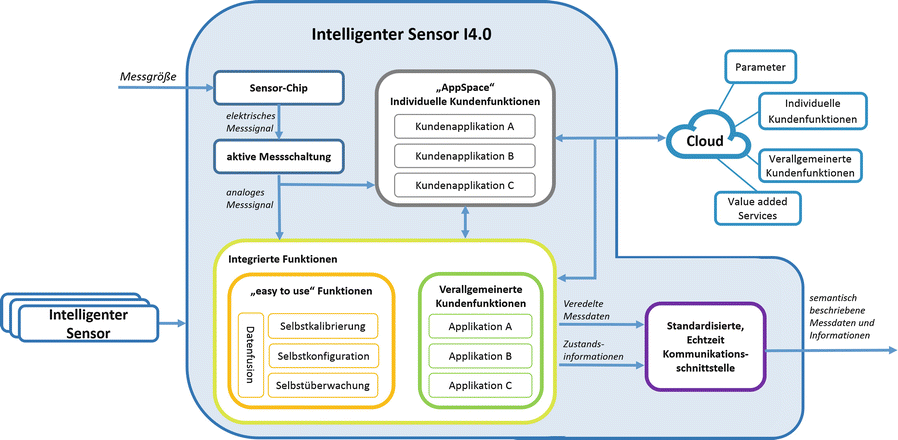
\includegraphics[scale=0.9]{picture/IntelligenterSensorSchema}
  \caption{Schema eines Intelligenten Sensors in einem CPS (Intelligente Sensorik als Grundbaustein für cyber-physische Systeme in der Logistik, Seite 11)}
  % [2] DOI: 10.1007/978-3-662-45537-1_83-1 Seite 11
 \label{fig:Schema eines Intelligenten Sensors in einem CPS } 
\end{figure}

\paragraph{Anforderungen eines Intelligente Sensoren für eine Anwendung in ein Cyber-physisches System \cite[Seite 14 ff.]{Furstenberg.2016}
}
\singlespacing
\begin{itemize}
\item \textit{echtzeitfähige} Kommunikationsschnittstelle um die ausgewertete Daten zu versenden.
\item Internetanbindung Informationen und Funktionen auszutauschen.
\item integrierte Funktionen für die Inbetriebnahme, Konfiguration, Parametrierung
automatisieren und die Wartbarkeit zu realisieren.
\item Sensor Signale von verschieden Quellen zu verarbeiten für
aufgewertete Messdaten.
\item Aufgaben eines Teilsystem unmittelbar auf dem Sensor zu Bewältigung.
\end{itemize}

\onehalfspacing
\subsubsection{Smartes Modul}
In verschiedenartigen Anwendungen werden Sensor-
Systeme bestehend aus einem oder mehreren Sensoren genutzt, um eine Aufgabe oder ein Dienst zu bewältigen. Diese Art von Sensornetzwerke wird auch als
„Smartes Modul“ bezeichnet, das Teil eines CPS, gleichzeitig mehrerer oder ein komplett autonomes CPS
sein kann.\\
Die Nutzung intelligenter Sensorik innerhalb eines smarten
Moduls ermöglicht sowohl die Wandelbarkeit als auch die schnelle Erweiterbarkeit eines CPS.\cite[Seite 15 ff.]{Furstenberg.2016}

% [2] DOI: 10.1007/978-3-662-45537-1_83-1 Seite 15 ff

\vspace{0.5cm}
% Define the layers to draw the diagram
\pgfdeclarelayer{background}
\pgfdeclarelayer{foreground}
\pgfsetlayers{background,main,foreground}

% Define block styles used later

\tikzstyle{sensor}=[draw, fill=blue!20, text width=5em, 
    text centered, minimum height=2.5em,drop shadow]
\tikzstyle{ann} = [above, text width=5em, text centered]
\tikzstyle{wa} = [sensor, text width=10em, fill=red!20, 
    minimum height=6em, rounded corners, drop shadow]
\tikzstyle{sc} = [sensor, text width=13em, fill=red!20, 
    minimum height=10em, rounded corners, drop shadow]

% Define distances for bordering
\def\blockdist{2.3}
\def\edgedist{2.5}

\begin{figure}[H]
\begin{tikzpicture}
    \node (wa) [wa]  {\large{Senkknoten}};
    \path (wa.west)+(-3.2,1.5) node (asr1) [sensor] {$Sensor_1$};
    \path (wa.west)+(-3.2,0.5) node (asr2)[sensor] {$Sensor_2$};
    \path (wa.west)+(-3.2,-1.0) node (dots)[ann] {$\vdots$}; 
    \path (wa.west)+(-3.2,-2.0) node (asr3)[sensor] {$Sensor_N$};    
   
    \path (wa.east)+(\blockdist,0) node (vote) [sensor] {$Aktor$\\Schnitt- stelle};

    \path [draw, ->] (asr1.east) -- node [above] {} 
        (wa.160) ;
    \path [draw, ->] (asr2.east) -- node [above] {} 
        (wa.180);
    \path [draw, ->] (asr3.east) -- node [above] {} 
        (wa.200);
    \path [draw, ->] (wa.east) -- node [above] {} 
        (vote.west);

               
    \path (wa.south) +(0,-\blockdist) node (asrs) {\Large{Smart Modul}};
  
    \begin{pgfonlayer}{background}
        \path (asr1.west |- asr1.north)+(-0.5,0.3) node (a) {};
        \path (wa.south -| wa.east)+(+0.5,-0.3) node (b) {};
        \path (vote.east |- asrs.east)+(+0.5,-0.5) node (c) {};
          
        \path[fill=yellow!20,rounded corners, draw=black!50, dashed]
            (a) rectangle (c);           
        \path (asr1.north west)+(-0.2,0.2) node (a) {};
            
    \end{pgfonlayer}
\end{tikzpicture}
\caption{Smart Modul (Intelligente Sensorik als Grundbaustein für cyber-physische Systeme in der Logistik, Seite 19)}
% [2] DOI: 10.1007/978-3-662-45537-1_83-1 Seite 19
 \label{fig:Smart Modul} 
\end{figure}

%[2] Intelligente Sensorik als Grundbaustein für cyber-physische Systeme in der Logistik DOI: 10.1007/978-3-662-45537-1_83-1

\newpage
\subsection{Kommunikation}
Wie in Abb. 3 schon illustriert ist die Kommunikation von komplexen Teilsystemen nicht mehr beschränkt auf Messdaten über einfache Bus-Systeme zu versenden sondern wird eine breitgefächerte Bidirektionale Austausch von Informationen. Anwender versenden über Server und Cloud-Systeme oder Bus-Systeme ihre Konfigurationsdaten in den intelligenten Sensor um Parameter zu verändern. Wobei wiederum der intelligente Sensor seine veredelten Daten zurück sendet.\\
\cite[14 ff.]{Furstenberg.2016}
Das schafft den einen Anwendungsspezifischen Sensor, der immer neu Konfigurierbar ist und auf Veränderungen eingestellt werden kann. IO-Link Sensoren sind dabei die Vorreiter solcher intelligenten Sensoren die durch Protokolle wie OPC/UA \& MQTT unterstützt werden. Diese Protokolle in der IKT bieten die Middleware zwischen der Steuerungsebene und Prozesssteuerung. Dabei steht ein sogenannter \textit{Broker} als OPC/UA Server und die Teilsysteme und Zentrale Einheiten als \textit{Subscriber} für eine Kommunikation im Netzwerk. Alle Teilsysteme können so per \textit{Topic} mithilfe MQTT in Nachrichten ihre Informationen weiterleiten.\\
Somit erreicht man eine neue Abstraktionsebene. Der Server oder die Zentrale Einheit eines CPS fordert Dienste im Server oder Cloud an. Wiederum werden die Anweisungen verschickt, von intelligenten Sensoren bewältigt und bereit gestellt.\cite[Seite 3 ff.]{Pr.Dr.DerkRembold.15.02.2019}
%[3] 
\vspace{0.5cm}

\begin{figure}[H]
\centering
\begin{adjustbox}{max width=\textwidth}
\begin{tikzpicture}[node distance=6cm,
    every node/.style={fill=white, font=\sffamily}, align=center]
  % Specification of nodes (position, etc.)
  \node (start) [activityStarts] {Dienst};
  \node (process)[process, right of=start]  {OPC/UA Server};
  \node (end)     [activityRuns, right of=process]   {Sensor};  
  % Specification of lines between nodes specified above
  % with aditional nodes for description 
  \draw[->]             (start) -- node[sloped] {\textit{MQTT}}(process);
  \draw[->]     		(process) -- node[sloped] {\textit{MQTT}}(end);
  \end{tikzpicture}
\end{adjustbox}
  \caption{Kommunikation zwischen Dienste und Intelligente Sensoren (Skript Digitale Fabrik Bussysteme und Middleware, Seite 11 ff.)}
 \label{fig:Kommunikation zwischen Dienste und Intelligente Sensoren} 
\end{figure}
  
% [2] DOI: 10.1007/978-3-662-45537-1_83-1 Seite 14 ff
% [3] Skript Digitale Fabrik Bussysteme und Middleware Seite 3 ff

\newpage
\subsubsection{Wireless Sensor Network}
Ein \textit{Wireless Sensor Network} besteht hauptsächlich aus drei Teilen, nämlich Sensorknoten, Senkknoten
und Aufgabenverwaltungsknoten.
Sensorknoten können entweder einfache oder intelligente Sensoren sein, die ihre aufbereiteten Daten an einen Senkknoten weiterführen. Schließlich kommen alle Daten in ein Aufgabenverwaltungsknoten der die Verwaltung des Teilsystems übernimmt.
Eine große Anzahl von Sensoren Knoten sind im Überwachungsbereich und im drahtlosen Kommunikationsnetz verteilt und übertragen Daten selbst organisiert an den Senkknoten. Nach Erhalt der Sensordaten, die von den Netzwerkknoten übertragen werden, leitet der Senkknoten die Daten an den
Verwaltungsknoten über ein MAC Protokoll weiter.
Sensorknoten verfügen über eine begrenzte Speicher- und Verarbeitungskapazität und die meisten Knoten sind nicht aktiv
um Strom zu sparen. Der Senkknoten
hat eine starke Verarbeitungsfähigkeit und Speicherkapazität. Der Aufgabenverwaltungsknoten kann die im Sensornetz gesammelten Daten empfangen und für den Weitertransport wie ein Gateway bereitstellen. Es können auch Steuerbefehle gesendet werden, um das gesamte Teilsystem per Broadcast zu konfigurieren und zu verwalten.\cite[Seite 128 ff]{FangTian.2018}
\vspace{0.5cm}
\begin{figure}[H]
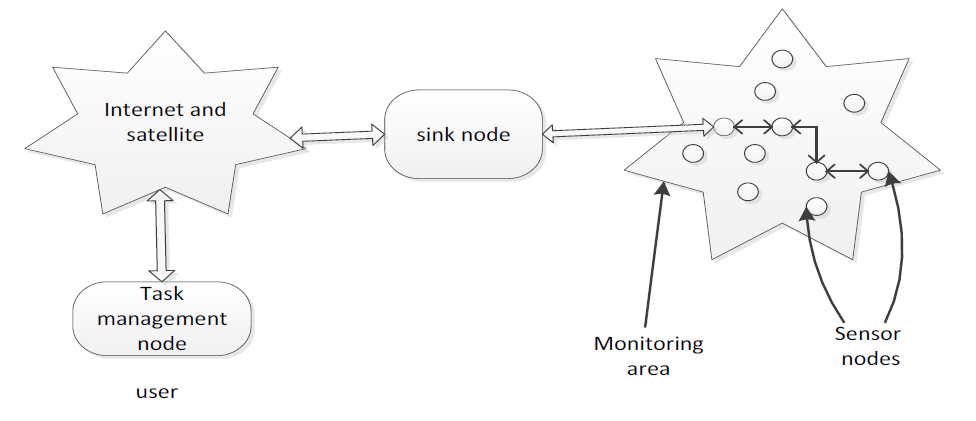
\includegraphics[scale=0.85]{picture/WSN}
\caption{Wireless Snesor Network Architektur (Design of Smart home System Based on Basic Radio Frequency Wireless Sensor Network Technologien 2022, Seite 128)}
\label{fig:Wireless Snesor Network Architektur}
\end{figure}

% [4] Design of Smart home System Based on Basic Radio Frequency Wireless Sensor Network Seite 128 ff
\section{Einsatzgebiete für Intelligente Sensoren}
Die Grundlagen von Sensoren und vor allem der Intelligenten Sensoren wurden hier nun erläutert. Die Kommunikation zwischen Intelligente Sensoren untereinander sowie mit Schnittstellen zu einem CPS oder dem Internet und Cloud Anwendungen sind selbstverständlich auch verfügbar.\\
Welches großes Ziel wird durch den Einsatz von intelligenten Sensoren angestrebt?\\ Die 4. Industrielle Revolution wartet. Diese „Wende“ wird durch die Informations-
und Kommunikationstechnologie ausgelöst und ändert den Aufbau von herkömmliche Prozesse komplett.
In diesem Kapitel präsentieren wir Beispielhafte Anwendungsbereiche von intelligente Sensoren im Bereich der Industrie.\cite[Seite 7 ff.]{VogelHeuser.2016}

\begin{figure}[H]
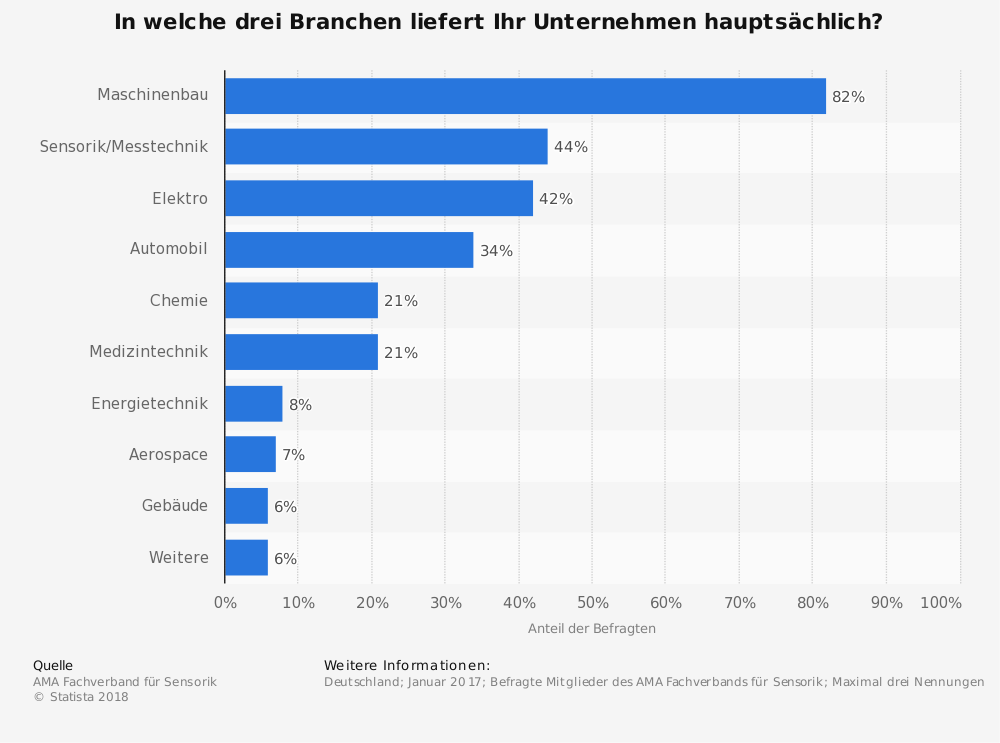
\includegraphics[scale=0.45]{picture/SensorikBranchen}
\caption{Sensorik - Umfrage zu den belieferten Branchen 2017 (Sensor Technologien 2022, Seite 11)}
\label{fig:Sensorik - Umfrage zu den belieferten Branchen 2017}
\end{figure}

%AMA Fachverband für Sensorik, Sensor Technologien 2022 Seite 11, November 2017

%[5] Handbuch Industrie 4.0 ISBN:978-3-662-53253-9 Seite 7 ff

\newpage
\subsection{Einsatz von Intelligente Sensoren in der Industrie}
Durch die digitale Revolution müssen Industrieunternehmen im Sinne von Industrie 4.0 teure noch verwendbare Maschinen aufrüsten mittels smarter Sensoren. 
In der Statistik Abb. 8 kann man sehr gut erkennen, dass der Absatz der smarten Sensoren in 10 Jahren um fast das 5-Fache steigen wird und somit unabdingbar für die Unternehmen sind.

\begin{figure}[H]
\centering
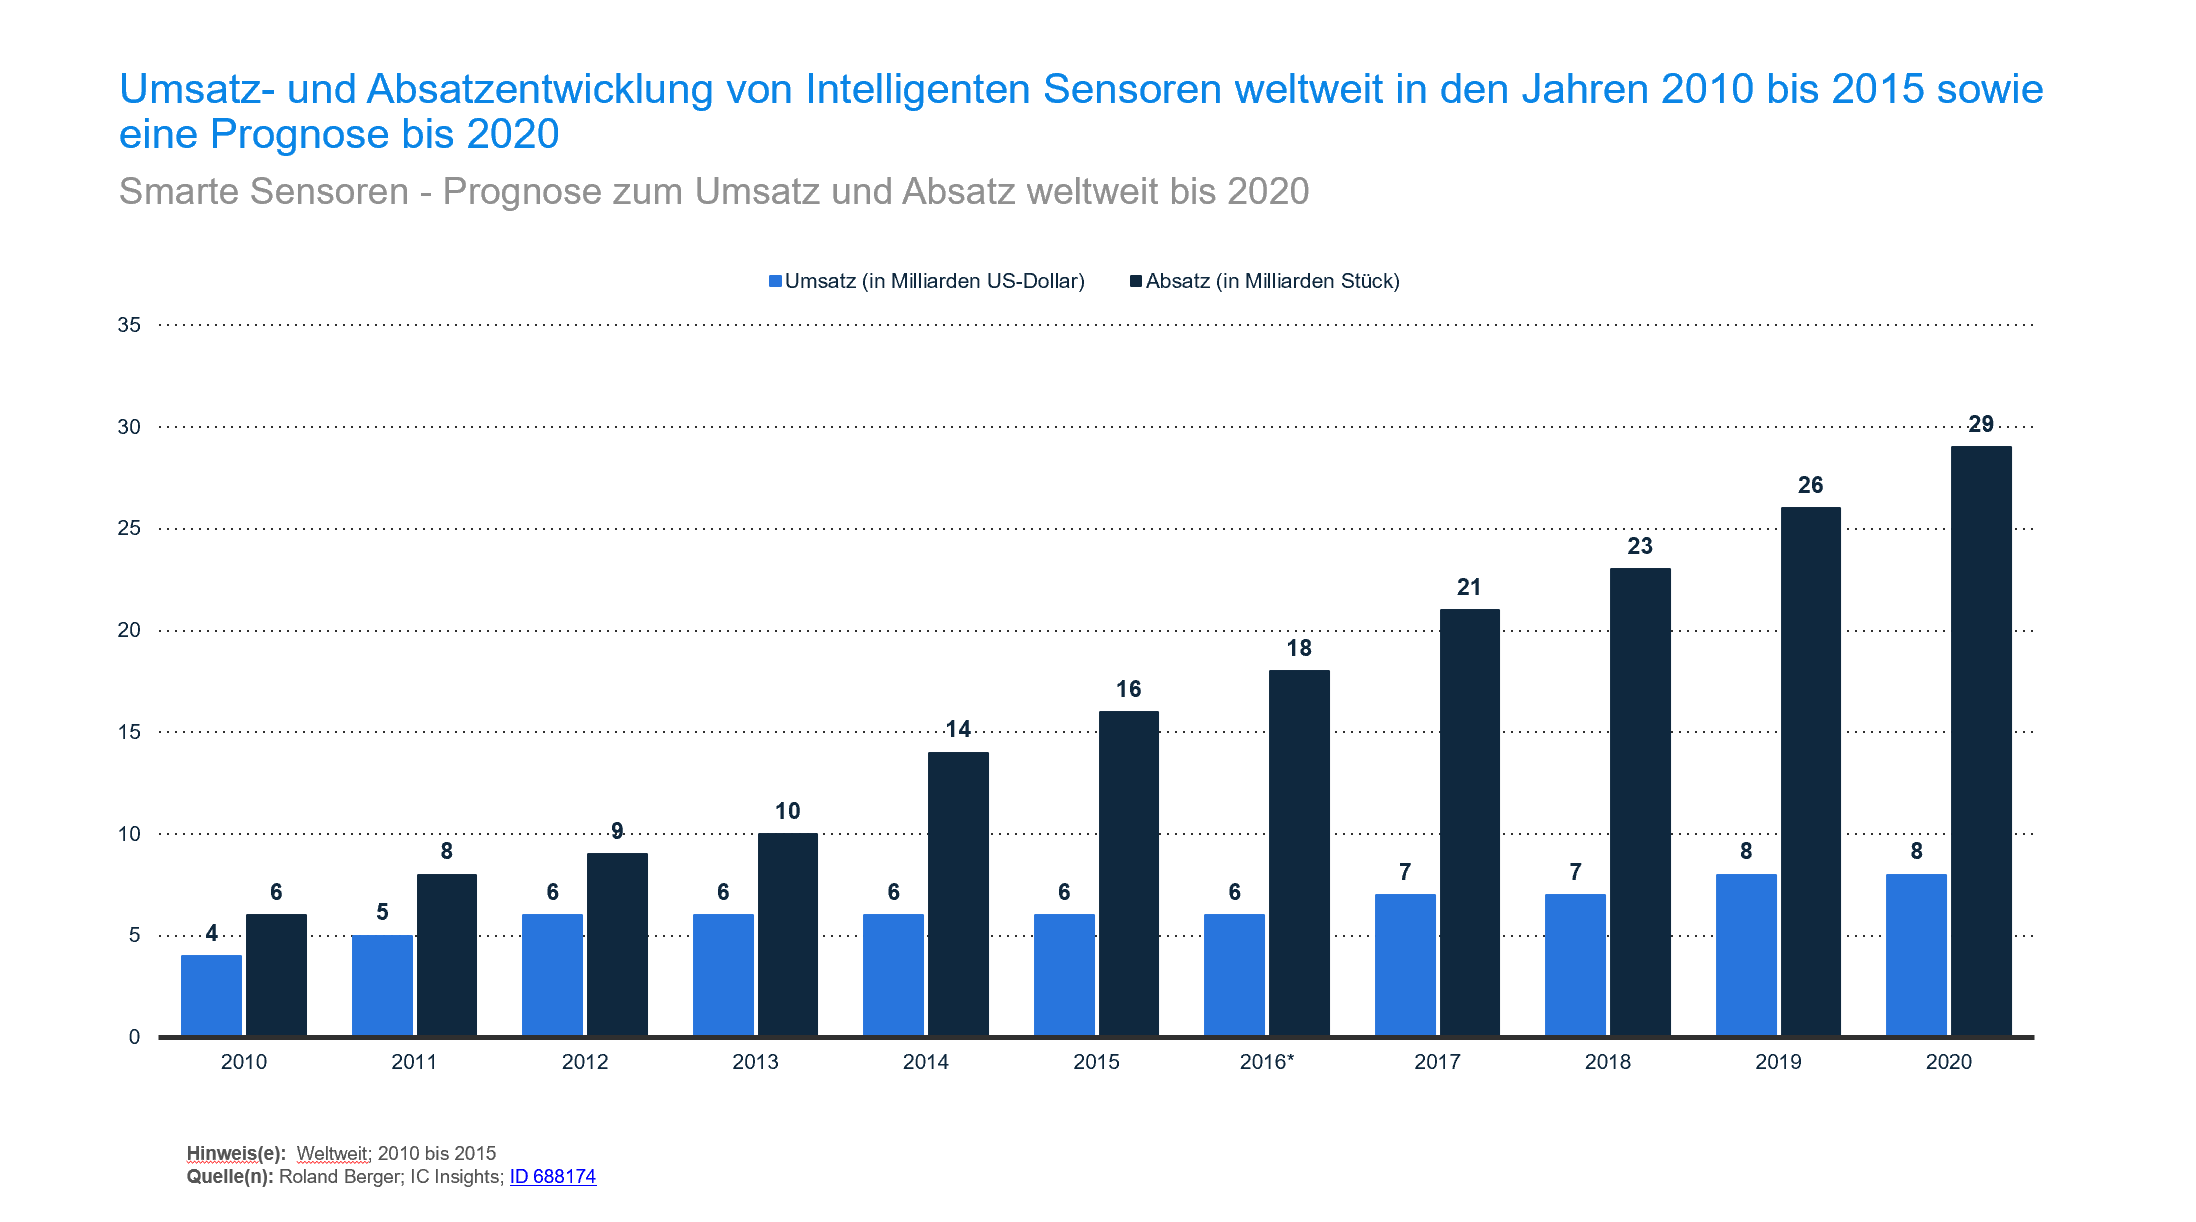
\includegraphics[scale=0.28]{picture/Prognose2020_1}
\caption{Umsatz- und Absatzentwicklung von Intelligenten Sensoren weltweit in den Jahren 2010 bis 2015 sowie eine Prognose bis 2020 (Umsatz- und Absatzentwicklung von Intelligenten Sensoren weltweit in den Jahren 2010 bis 2015 sowie eine Prognose bis 2020, Folie 4))}
\label{fig:Umsatz- und Absatzentwicklung von Intelligenten Sensoren weltweit in den Jahren 2010 bis 2015 Balkendiagramm}
\end{figure}

Hierbei kann bspw. der Sensor eines herkömmlichen Thermostates an einer Maschine so aufgerüstet werden, dass dieser statt nur der Anzeige von warm/kalt, die expliziten Messdaten an eine IoT-Plattform versendet, ab dem z.B. die Temperatur der Maschine 40 Grad erreicht hat welches zuvor festgelegt wurde.\cite{ComarchAG.}

\subsubsection{Anwendungsbeispiel am RFID}
Das erste Anwendungsbeispiel ist der RFID-Transponder. Dieser wird in der Industrie immer häufiger zum Einsatz gebracht und funktioniert folgender maßen. 
Es gibt 4 verschiedene Arten der Kopplung von RFID, LF, HF, UHF und Mikrowellen. 
Bei der Kopplung über LF RFID findet die Kopplung über Spulen statt. So kann ein Lesegerät ein Magnetfeld erzeugen und der jeweilige Transponder entzieht aus dem Magnetfeld Energie. Der Frequenzbereich ist hierbei 125-135 kHz.

\begin{figure}[H]
\centering
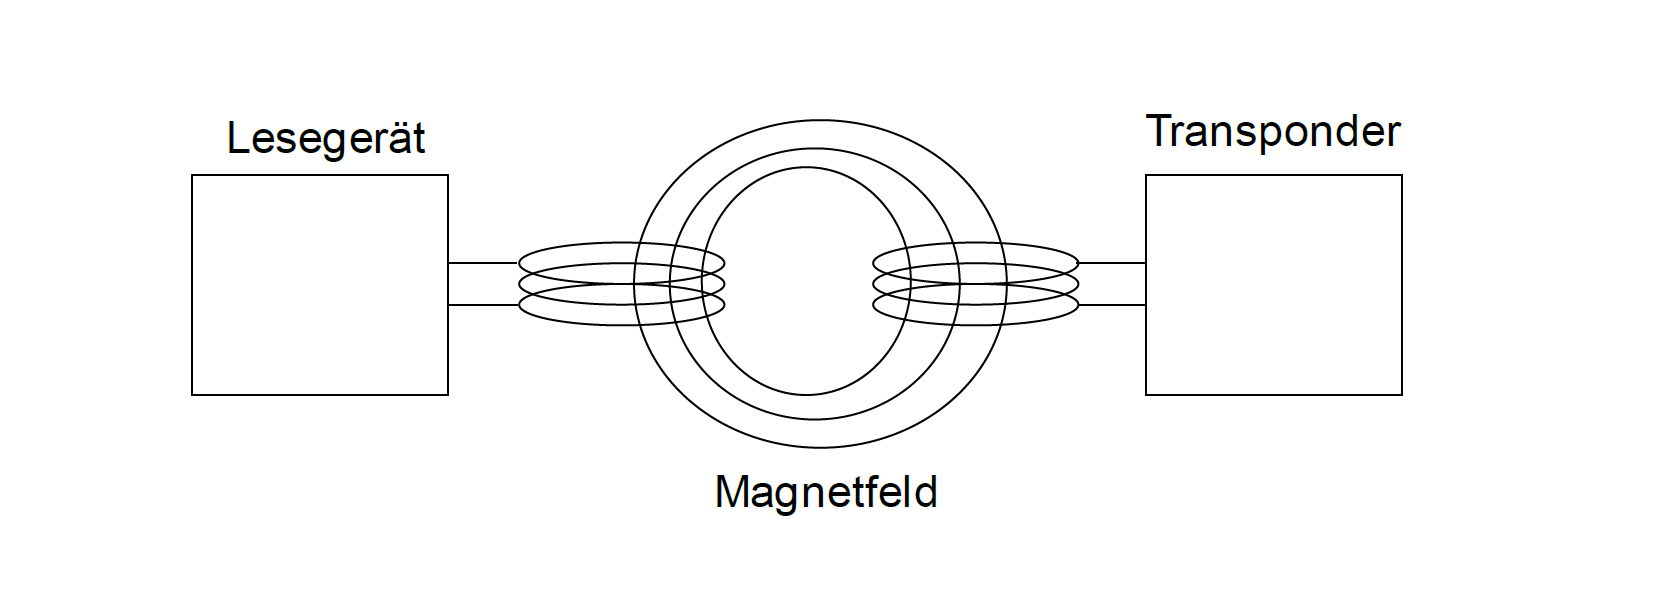
\includegraphics[scale=0.28]{picture/rfid}
\caption{Funktionsweise eines RFID (Skript Digitale Fabrik(DF): Autoidentifikation von Prof. Dr. Derk Rembold, Seite 15))}
\label{fig:Funktionsweise eines RFID}
\end{figure}

Mittels HF/UHF RFID sendet der Sender eine elektromagnetische Welle an den Empfänger. Der Empfänger nimmt es an und reflektiert es mit der Modulation der Information über die Reflektionseigenschaften. Der Sender empfängt danach wieder die reflektierte Welle und demoduliert sie. Der Frequenzbereich beträgt hierbei bei HF 13,56 MHz und bei UHF 433 und 868 MHz.

\begin{figure}[H]
\centering
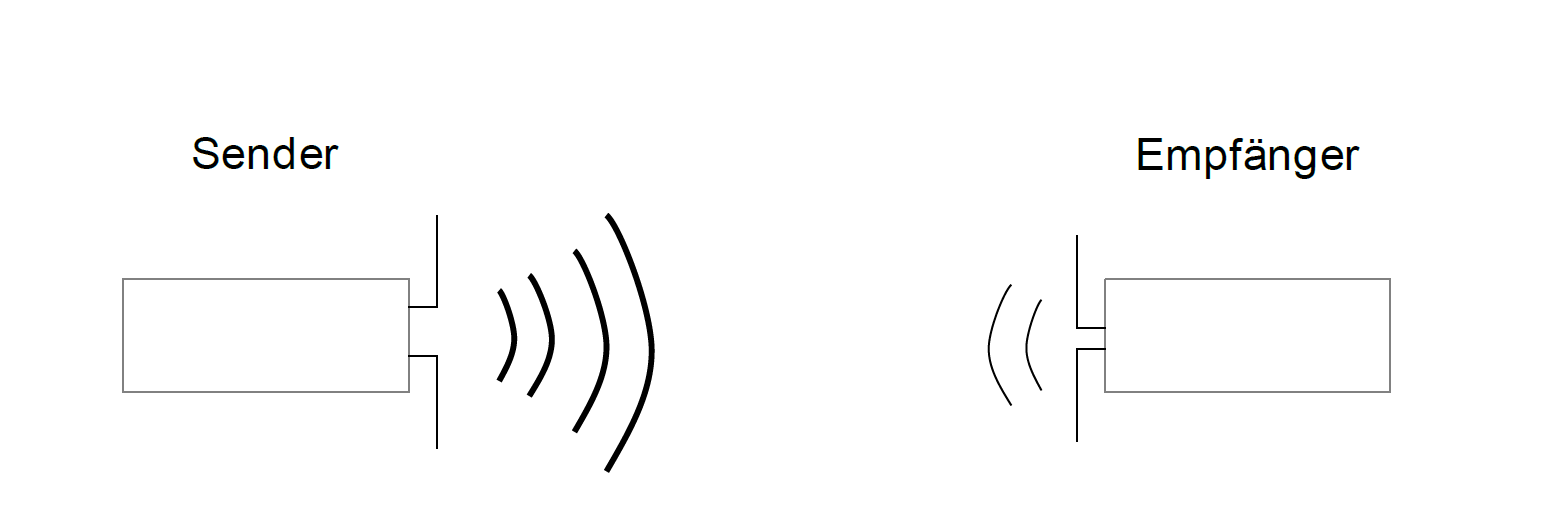
\includegraphics[scale=0.28]{picture/kopplung}
\caption{Kopplungsweise eines RFID Sensors (Skript Digitale Fabrik(DF): Autoidentifikation von Prof. Dr. Derk Rembold, Seite 16))}
\label{fig:Kopplungsweise eines RFID Sensors}
\end{figure}

Mit der letzten RFID Art erzeugt ein Frequenzgenerator eine Referenzsinuswelle. Hierbei werden die Informationen auf moduliert und danach mit der Antenne als elektromagnetische Welle abgegeben. Der Empfänger auf der Gegenseite nimmt diese Welle auf und ladet somit den Kondensator zur Spannungsversorgung. Daraufhin kann das Signal demoduliert werden. Der Frequenzbereich beträgt hierbei 2,45 GHz.

\begin{figure}[H]
\centering
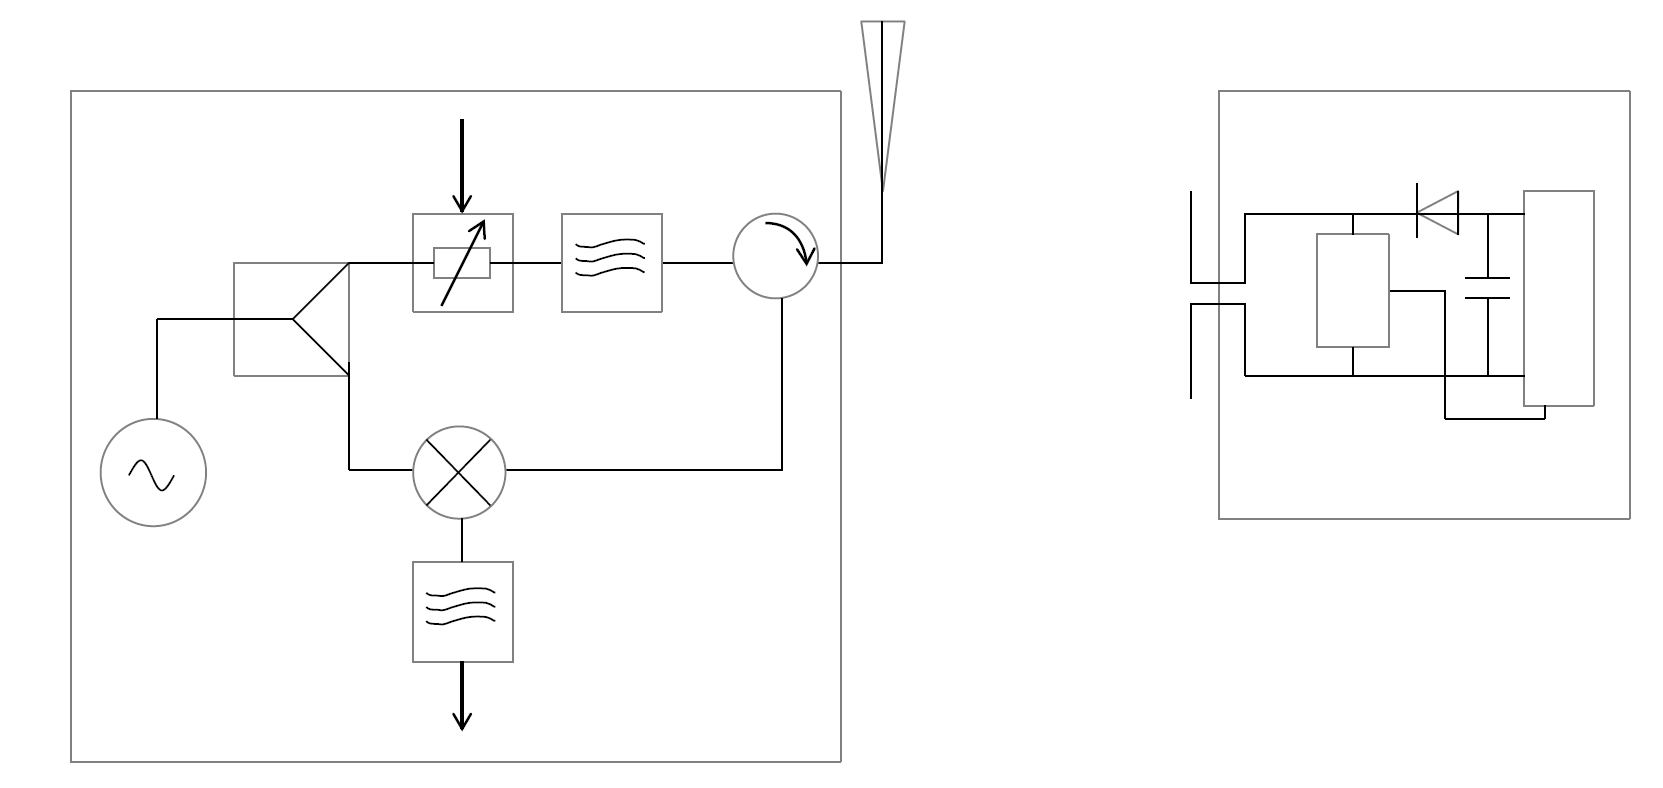
\includegraphics[scale=0.28]{picture/mikrowellen}
\caption{Passive Kopplung durch Mikrowellen eines RFID Sensors (Skript Digitale Fabrik(DF): Autoidentifikation von Prof. Dr. Derk Rembold, Seite 17))}
\label{fig:Passive Kopplung durch Mikrowellen eines RFID Sensors}
\end{figure}

\paragraph{Spezifisches Beispiele am RFID
\cite{IndustrieundHandelskammerReutlingen.}}

\singlespacing
\begin{itemize}
\item \textbf{Warenlieferung}\\
Mithilfe von RFID kann schnell und vollautomatisch angelieferte Waren durch Pulkererfassung registriert und identifiziert werden. Durch die ID einer gelieferten Palette hat das Handelsunternehmen die Möglichkeit Waren automatisch zu vereinnahmen. Dies hat den Vorteil, dass aufwändige Zähl-, Such- und Sortierungsprozesse nicht mehr nötig sind und man dadurch sehr viele Kosten und auch Zeit einsparen kann. Durch diese Vollautomatisierung bekommt sowohl der Hersteller als auch das Unternehmen, welches die Waren annimmt, eine Empfangsbestätigung der Ware.
\item \textbf{Lagermanagement}\\
Durch die RFID Technologie im Lagersystem ist man in der Lage jederzeit die aktuelle Anzahl von Produkten, als auch den Ort der Ware zu ermitteln. Dadurch kann man Probleme im Sinne von Produktengpässen vermeiden und Platz sparen, da es zu keiner Überproduktion kommen kann.
\item \textbf{Intelligente Regale}\\
Aufgrund der Lesegeräte an den Regalen kann automatisch jegliche Veränderung der Ware erfasst werden. Dies beinhaltet Punkte wie Entnahme und Befüllung der Ware, Temperatur der Ware oder die Zeit wie lange die Ware schon aufbewahrt wird. Dies hat den Vorteil, dass man anhand dieser Messdaten bei einer Produktionslinien von beispielsweise Käse oder Whisky die Qualität bestimmen kann.
\item \textbf{Tracking and Tracing}\\
Durch die jeweilige UID eines Produktes hat man die Chance jeden Prozess individuell Rückzuverfolgung. Somit kann man genau sagen welche Transportwege ein Produkt durchlaufen ist und kann bei Fehleranalyse direkt ausfindig gemacht werden.
\item \textbf{Diebstahlsicherung}\\
Mithilfe des Transponders auf jedem Produkt und jeder Ware hat man die Chance zu sehen ob eine Ware einen bestimmten Bereich unerlaubt verlässt in dem man direkt eine Meldung am jeweiligen Gerät bekommt. Dadurch wird der Faktor Diebstahl dezimiert. 
\end{itemize}
\onehalfspacing

\newpage
Wie wichtig RFID-Transponder seit dem Jahre 2010 sind kann man ebenfalls an Abb. 12 erkennen.

\begin{figure}[H]
\centering
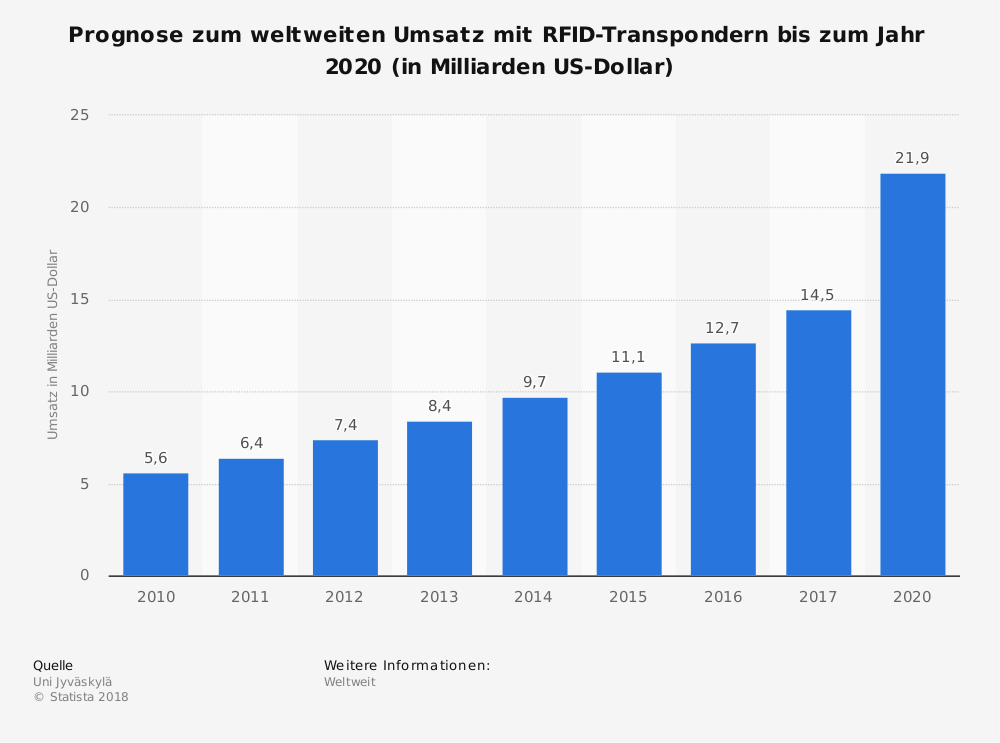
\includegraphics[scale=0.45]{picture/prognoserfid}
\caption{Prognose zum weltweiten Umsatz mit RFID-Transpondern bis zum Jahr 2020 (Internet-of-Things Market, Value Networks, and Business Models: State of the Art Report 2013, Seite 16)}
\label{fig:Prognose Umsatz RFID Sensors}
\end{figure}

Dabei erkennt man das laut der Prognose der Statista der Umsatz um das ca. 4-Fache steigen wird in einem Zeitraum von 10 Jahren.

\newpage
\subsubsection{Anwendungsbeispiel Autonomes Fahren}
Heutzutage ist dank der industriellen Revolution ein Kraftfahrzeug nicht mehr eine rein mechanische Maschine, welche voll und ganz die Unterstützung des Endnutzers benötigt. Zur heutigen Zeit sind wir durch zum Teil smarte Sensoren schon beinahe soweit, dass die Autos aufgrund dieser selbständig fahren können.
Hierbei zähle ich 4 Smart-Sensoren für die äußere Umgebung eines Fahrzeuges auf.
Zum einen gibt es hier zum Parken einen Ultraschallsensor, der die Hindernisse rund ums Fahrzeug erfasst und am Bordcomputer anzeigt ob diese zu nah oder zu fern am Fahrzeug sind.
Der Nahbereichsradar ist vor allem während der Fahrt ein echter Lebensretter. Dieser erfasst bis zu einem bestimmten Radius des Autos Objekte, die eine Kollision verursachen könnten. Dies hat den Vorteil, dass die Sicherheitssysteme des Fahrzeuges schnell aktiv gesetzt werden und somit jeglichen Schaden auf das geringfügigste reduzieren werden kann.
Auch Bildsensoren spielen eine Rolle wenn es um Komfort geht. Diese ermöglichen es das Fahrzeug zum Großteil selbständig zu fahren. Der Sensor ist fähig eigenständig Verkehrsschilder zu erkennen und diese am Bordcomputer anzuzeigen. Des Weiteren kann es Fahrbahnkonturen erkennen und somit den Fahrer vor gefährlichen Abweichungen warnen und auch teilweise selbständig zu fahren.
Der Weitbreichs-Radarsensor ermöglicht es dem Fahrer auch bei schlechten Wetterbedingungen ca. 150 m weit jegliche Hindernisse und Gefahren zu erkennen, zu melden und gegeben falls langfristig eigenständig zu fahren.
\cite[Seite 15]{Reif.2012}
\\

\newpage
\subsection{Intelligente Sensoren in der Landwirtschaft}
Ein weiterer Zweig der Industrie, an dem man den nutzen der intelligenten Sensoren gut erkennen kann, ist die Landwirtschaft. 
Von Farmen wird erwartet, in immer kürzerer Zeit immer mehr und immer hochwertigere Produkte zu liefern. So sollen Farmen bis 2050 über 9.8 Milliarden Menschen ernähren können.
\cite[Seite 21]{King.2017}
%\cite{Technology: The Future of Agriculture Seite 21}\\

Dies würde bedeuten, dass die Nahrungserträge um 70\% erhöht werden müssten. \cite[Seite 1]{Navulur.2017}
Diese Aufgabe ist aufgrund von steigendem Platzmangel nur durch technische Hilfsmittel erreichbar. Schon heute wird die Landwirtschaft von digitalen Werkzeugen, Sensoren und überwachenden Prozessen unterstützt.

\cite[Seite 1]{RaminShamshiri.2018}\\

Dieser Trend wird sich in Zukunft noch weiter vorsetzen, daher wird oft von Landwirtschaft 4.0 in Anlehnung auf Industrie 4.0 gesprochen.

\subsubsection{Anwendungsbeispiel in der Landwirtschaft}
In dieser Landwirtschaft 4.0 spielen, wie schon erwähnt, Sensoren eine sehr wichtige Rolle. So wird schon heute Beispielsweiße auf den Feldern die Bodenqualität, die Feuchtigkeit der Luft und die Temperatur erfasst. Dadurch lassen sich bereits frühzeitig Probleme wie Krankheiten und Pilzbefall an den Pflanzen erkennen. Auch die optimalen Zeiten zum sähen und ernten der Pflanzen lassen sich so bestimmen. Auch in anderen Bereichen der Landwirtschaft haben die Sensoren bereits Einzug gefunden. So werden Treibhäuser häufig überwacht. Es werden die CO2-Werte, die Temperatur, die Luftfeuchtigkeit und vieles mehr genaustens beobachtet.

\cite[Seite 2]{Navulur.2017}\\


Selbst in der Tierzucht sind Sensoren eine sehr große Hilfe. Es gibt bereits erste Projekte, in denen Kühe per Sensor überwacht werden. Hierfür wird der Sensor an ihren Köpfen befestigt. Dort misst er dann die Bewegungen der Kuh und ihre Körpertemperatur. Daraus lässt sich schließen, in welchen Gesundheitlichen zustand sich das Tier befindet. Diese Daten lassen sich dann direkt auf einem Computer oder Smartphone anzeigen.

\cite{Cowlar.}

\subsubsection{Spezifisches Beispiel in der Landwirtschaft}
Bei den meisten bisher gennannten Beispielen handelt es ich jedoch um gewöhnliche Sensoren. Dennoch liegt die Zukunft auch hier, in der Landwirtschaft 4.0, bei den smarten Sensoren.
Die ersten Projekte, die diese schlauen Sensoren benutzen sind bereits auf den Markt erschienen. Ein sehr gutes Beispiel hierfür ist Pycno. Bei Pycno handelt es sich um eine Erweiterung der schon erwähnten Feldüberwachung. 
Pycno besteht aus mehreren einzelnen Sensoren, die sich über Solaranlagen aufladen können und dazu in der Lage sind, miteinander zu kommunizieren. Die einzelnen Sensoren werden in den Boden gesteckt. Durch den Teil des Sensors, der sich im Boden befindet, kann per kapazitiven Feuchtigkeitssensor erkannt werden, wie feucht die Erde ist. Zusätzlich wird die Temperatur der Erde erfasst. Am oberen Ende befinden sich weitere Sensoren, die die Temperatur und Luftfeuchtigkeit messen können. Diese erfassten Daten werden dann in einem Netzwerk unter den verschiedenen Knoten-Sensoren an den einzigartigen Master-Sensor weitergeleitet. Bei dem Master-Sensor handelt es sich um den Sensor, der tatsächlich mit dem Internet verbunden ist. Die restlichen Knoten-Sensoren sind nur indirekt mit dem Internet verbunden. In diesem Master-Sensor werden die Daten gesammelt, aufgewertet und abschließend an den Nutzer weitergeleitet.
In diesem WSN soll es in Zukunft ebenfalls möglich, eine Selbstüberwachung der Sensoren auszuführen, um so frühzeitig und direkt Fehler von einzelnen Sensoren erkennen zu können. Dies stellt eine vereinfachte Form der Predictive Maintenance dar.

\cite{Pycno.}
%\cite{https://pycno.co/quick-start Stand 14.02.2019, 14:00 Uhr }

\begin{figure}[H]
\centering
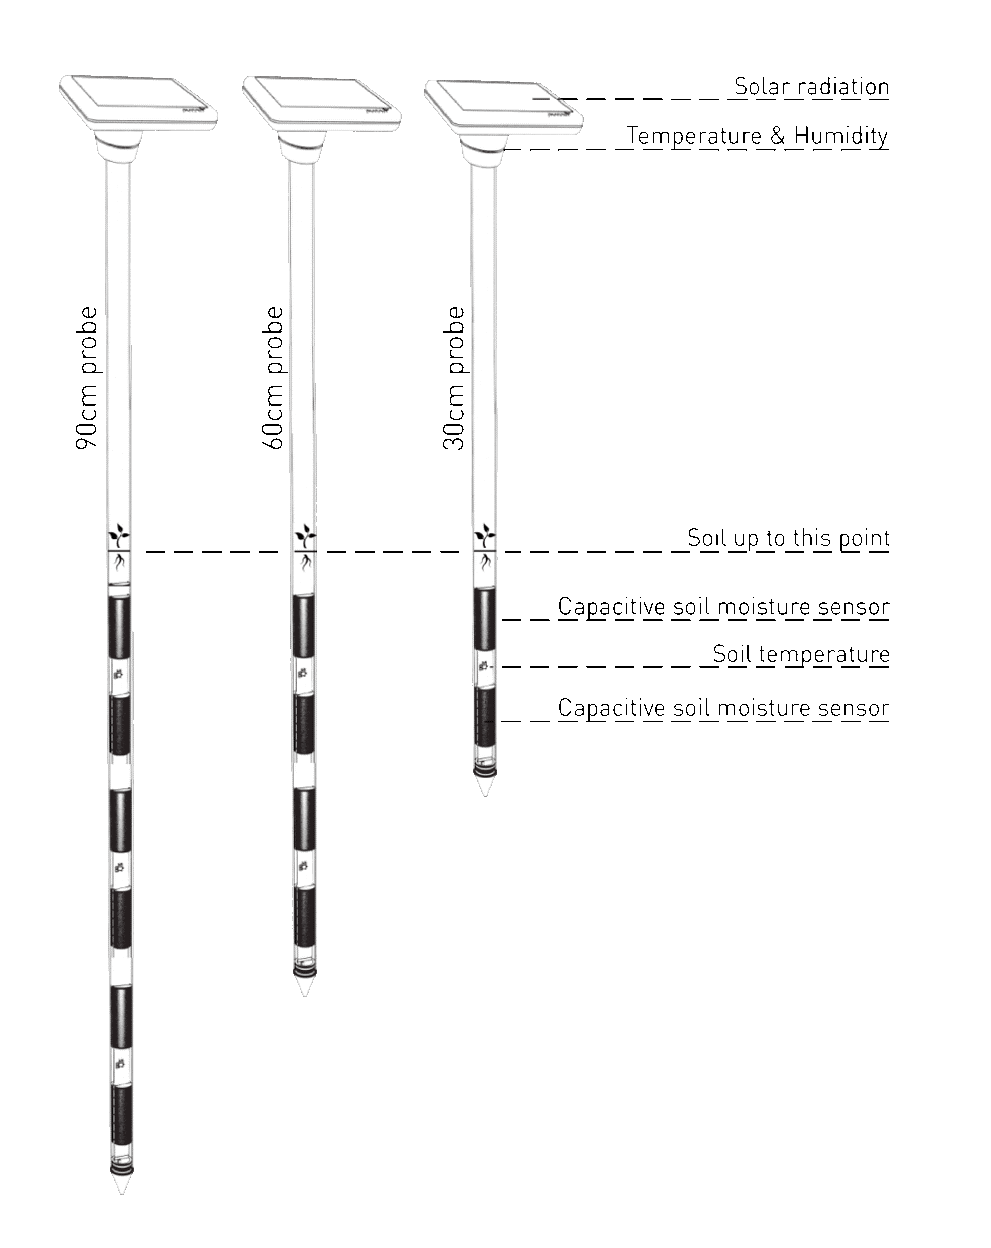
\includegraphics[scale=0.4]{picture/pycno}
\caption{Aufbau der Sensoren der Firma Pycno (https://pycno.co/quick-start Stand 14.02.2019, 14:00 Uhr)}
\label{fig:Aufbau der Sensoren der Firma Pycno}
\end{figure}

\newpage
\subsubsection{Fazit zu Intelligenten Sensoren in der Landwirtschaft}
Insgesamt lässt sich zusammenfassen, dass intelligente Sensoren in der Landwirtschaft eine sehr große Zukunft haben werden. Dennoch muss man dazu sagen, dass viele Landwirte sich noch nicht mit der Idee von Sensoren angefreundet haben. So haben gerade einmal 26\% insgesamt für die Zukunft geplant, ihre Arbeit mit Sensoren zu vereinfachen.

\begin{figure}[H]
\centering
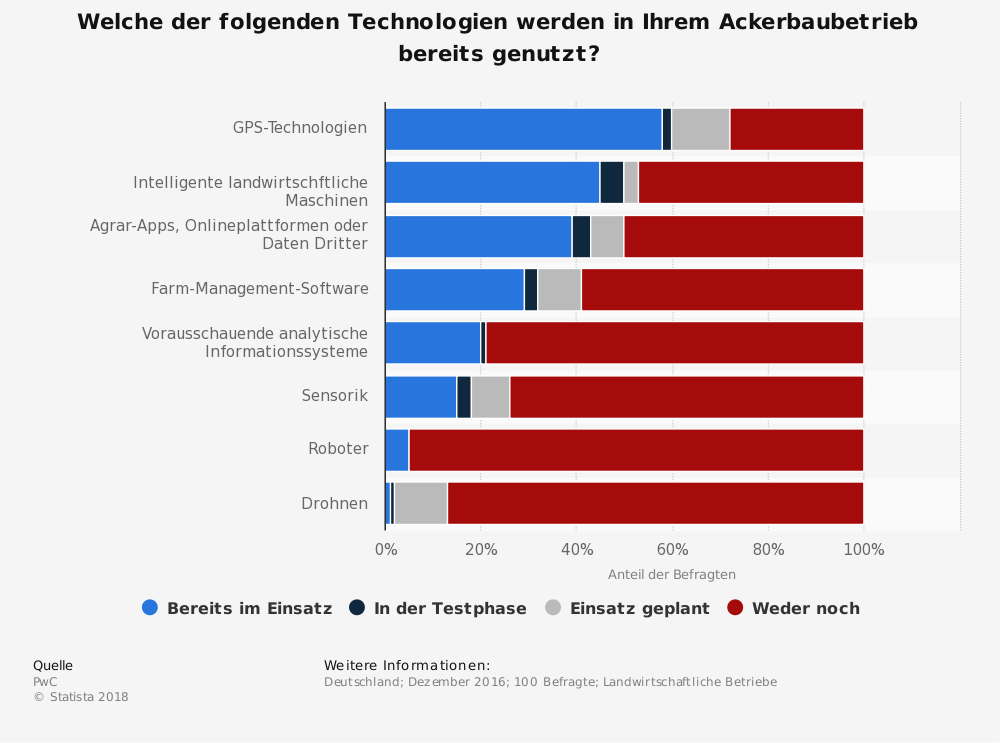
\includegraphics[scale=0.45]{picture/Landwirtschaft}
\caption{Landwirtschaft 4.0 - Umfrage zur Nutzung neuer Technologien in Deutschland 2016 (PwC - Quo vadis, agricola?, Seite 12)}
\label{fig:Landwirtschaft 4.0 - Umfrage zur Nutzung neuer Technologien in Deutschland 2016}
\end{figure}

Dies lässt sich jedoch auf die Neuheit des Themas zurückführen. So werden erst seit etwa 2010 aktiv Daten in der Landwirtschaft per Sensoren erfasst.
\cite[Seite 6]{Navulur.2017}

Mit großer Wahrscheinlichkeit wird auch in diesem Bereich der Industrie der Absatz von Sensoren stark steigen, sobald diese sich bewiesen haben.
\cite{ComarchAG.}

\newpage
\subsection{Intelligente Sensoren in der Forschung}
Intelligente Sensoren werden neben der Industrie auch noch in vielen anderen Bereichen eingesetzt. Ein sehr vielversprechendes Einsatzgebiet hierbei ist die Forschung. Speziell in der Überwachung spielt die schnelle und dezentrale Verarbeitung von Daten eine sehr wichtige Rolle. Daher ist es nicht verwunderlich, dass Katastrophen die üblicherweise mit normalen Sensoren überwacht werden eine sinnvolle Möglichkeit sind, intelligenten Sensoren zu nutzen. 

\subsubsection{Anwendungsbeispiel Tsunami}
So werden Beispielsweiße in den USA bereits kleine Netzwerke von Sensoren eingesetzt, um vor Tsunami-Katastrophen zu schützen. Da diese jedoch über Satelliten miteinander kommunizieren und eine externe Auswertung benötigen, verschwendet dies kostbare Zeit in einem Ernstfall. Die alternative hierfür wäre ein Netz aus Sensoren, welches nicht über Satelliten, sondern direkt untereinander per Radio Frequenz kommunizieren. Zusätzlich hierzu würde es einige ausgewählte Sensoren geben, welche die gesammelten Daten auswerten. Diese Methode würde mehr Sensoren benötigen, dadurch würde jedoch die Reaktionszeit deutlich verbessert werden.
Unabhängig der Überwachungsart, die Funktionsweiße der Sensoren bleibt jedoch dieselbe. Bei den Sensoren handelt es sich um Seismographen. Mithilfe dieser lassen sich leichte Erschütterungen auf dem Meeresboden erkennen. Da diese meist die Verursacher von Tsunamis sind, können diese Daten genutzt werden, um ein Tsunami frühzeitig zu erkennen. Ebenfalls wird die Höhe des Meeresspiegels zur Bestimmung miteinbezogen. Diese Daten werden daraufhin ausgewertet umso zu entscheiden, ob es sich um einen Ernstfall handelt, oder nicht. 
\cite[Seite 3 ff.]{Casey.2008}

\begin{figure}[H]
\centering
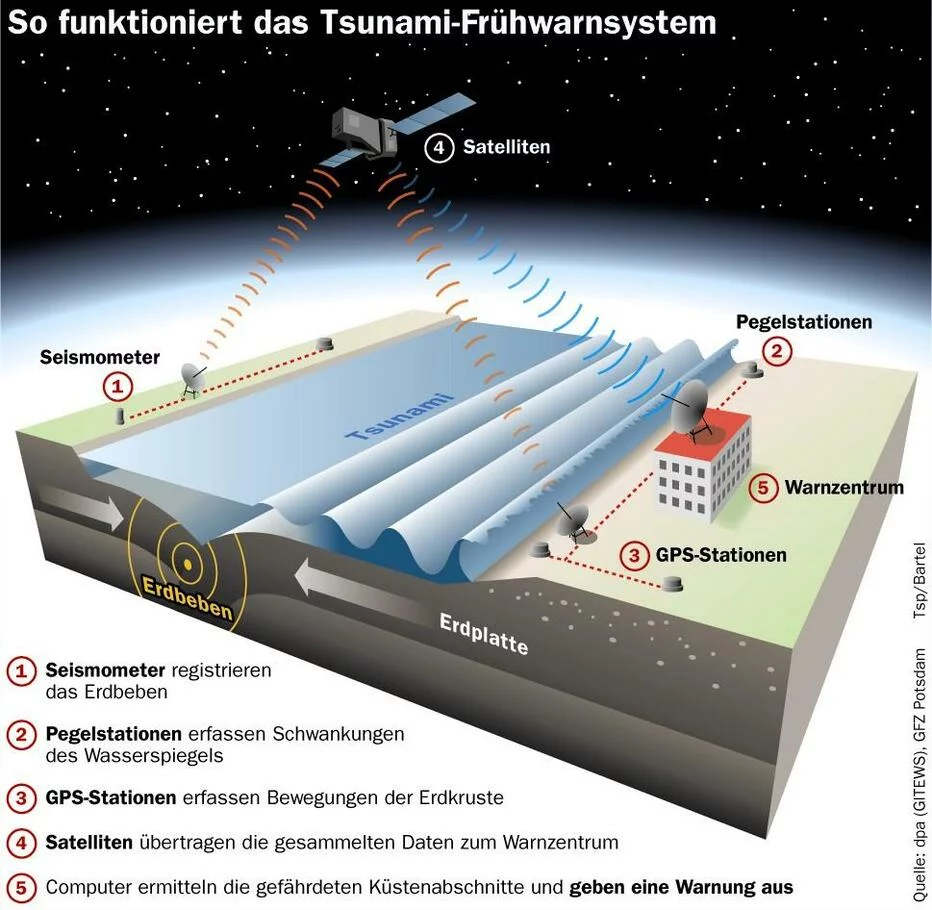
\includegraphics[scale=0.6]{picture/tsunami}
\caption{Funktion des aktuellen Frühwarnsystems (GITEWS/DPA/TSP)}
\label{fig:Funktion des aktuellen Fruehwarnsystems}
\end{figure}

Auch in diesen Bereich können intelligente Sensoren mehr erreichen als normale Sensoren. In diesem Fall könnten dank der schnelleren Reaktionszeit sogar Leben gerettet werden. Statistiken weißen deutlich darauf hin, dass Tsunamis zu einen der Häufigsten und gefährlichsten Naturkatastrophen überhaupt gehören, sowohl was Sachschäden als auch Menschenleben betrifft. Daher ist es wichtig jegliche Mittel zu nutzen, um diese Frühzeitig zu erkennen und mögliche Schäden zu minimieren.

\begin{figure}[H]
\centering
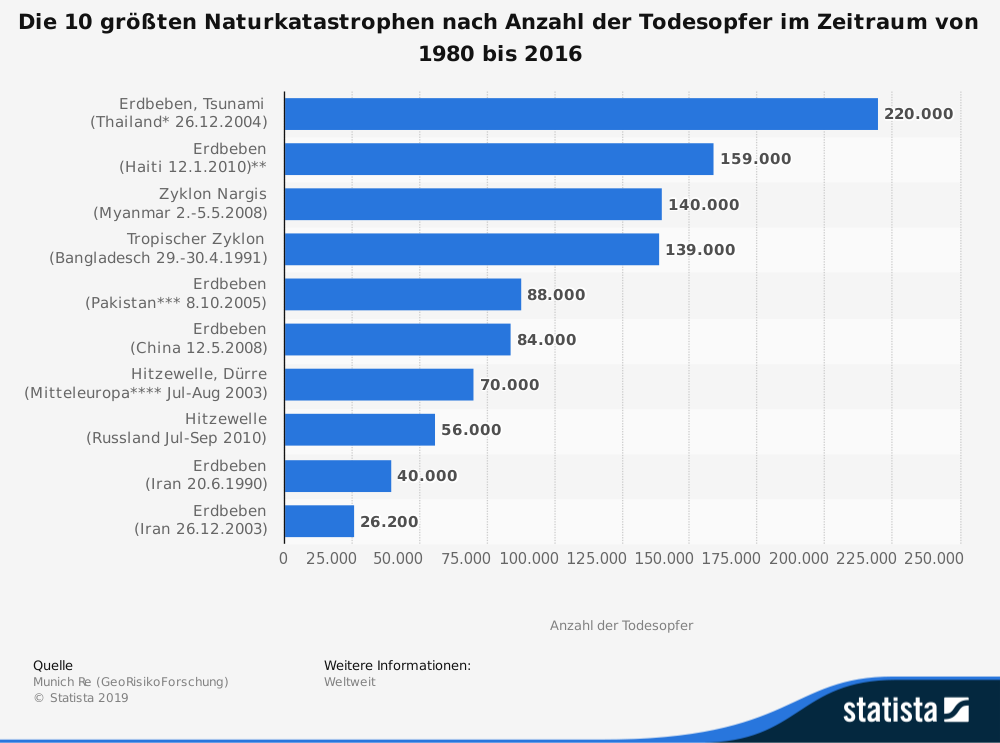
\includegraphics[scale=0.45]{picture/opfer}
\caption{Größte Naturkatastrophen nach Anzahl der Todesopfer bis 2016 (Munich Re (GeoRisikoForschung))}
\label{fig:Anzahl der Todesopfer durch Tsunami bis 2016}
\end{figure}

\newpage
\section{Zukunftsaussichten}
\subsection{Marktentwicklung}
Smarte Sensoren sind ein explosionsartig wachsender Markt. So haben sich die Absatzzahlen für intelligente Sensoren allein im Zeitraum von 2010 bis 2015 verdreifacht und sind prognostiziert bis 2020 auf 29 Milliarden Verkaufte Einheiten pro Jahr zu steigen. Umsatzzahlen dagegen sind im gleichen Zeitraum nur mit dem Faktor 1,5 gestiegen (Abb. 17). Dies zeigt deutlich die Popularität und die Besserung der Preise, was zur noch stärkeren Verbreitung der Technologie führen sollte. 
 
\begin{figure}[H]
\centering
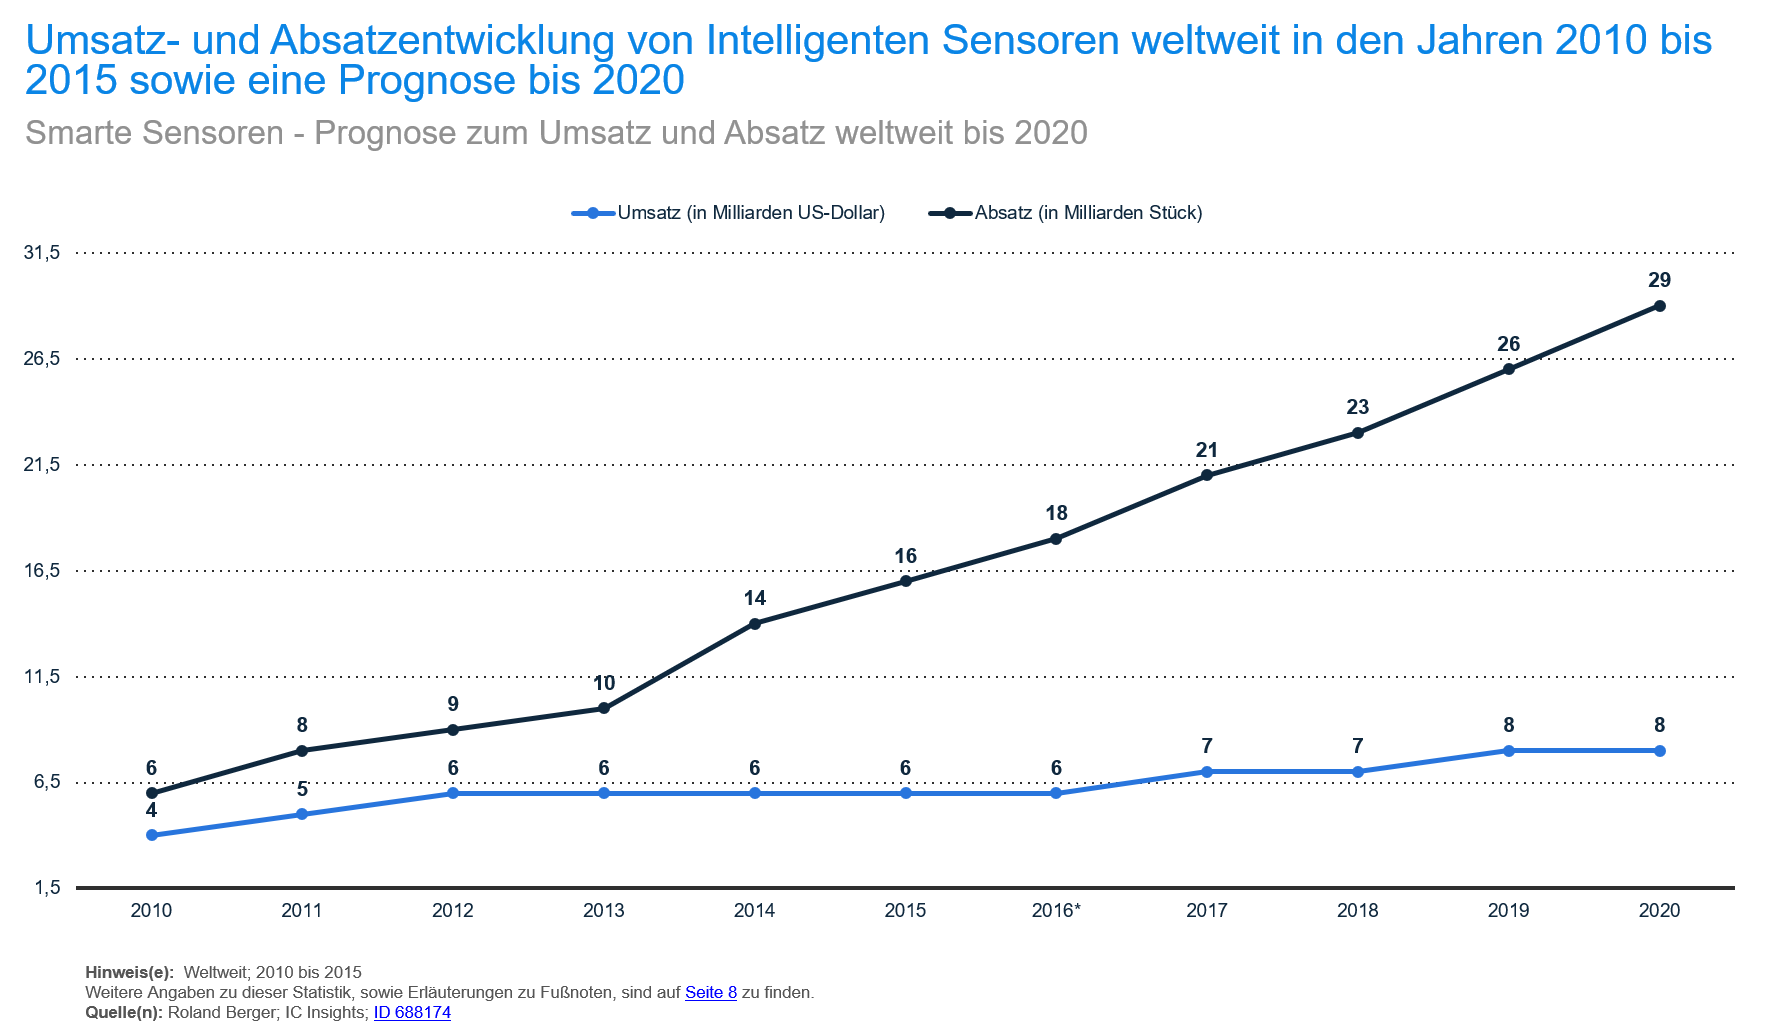
\includegraphics[scale=0.50]{picture/Prognose2020}
\caption{Umsatz- und Absatzentwicklung von Intelligenten Sensoren weltweit in den Jahren 2010 bis 2015 sowie eine Prognose bis 2020 (Umsatz- und Absatzentwicklung von Intelligenten Sensoren weltweit in den Jahren 2010 bis 2015 sowie eine Prognose bis 2020, Folie 6)}
\label{fig:Umsatz- und Absatzentwicklung von Intelligenten Sensoren weltweit in den Jahren 2010 bis 2015 sowie eine Prognose bis 2020}
\end{figure}

In einer Studie 2017 gaben 39\% der befragten Unternehmen an dass sie bereits Verbundene Sensoren in Betrieb haben und ganze 64\% planen die zukünftige Nutzung. Damit sind smarte Sensoren eine der beliebtesten Innovationsmöglichkeiten und lassen Techniken wie 3D-Druck und Virtuelle Realität weit hinter sich (Abbildung 18).\\

\begin{figure}[H]
\centering
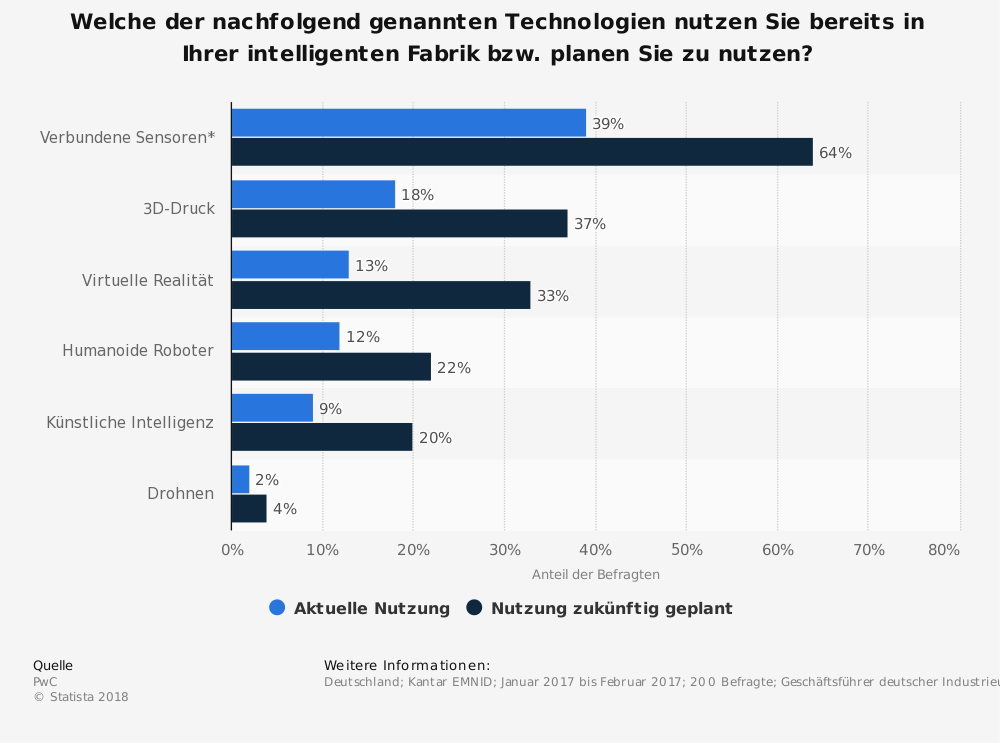
\includegraphics[scale=0.45]{picture/SensorikBereiche}
\caption{Smart Factory - Genutzte Technologien in Deutschland 2017 (Digital Factories 2020, Seite 24)}
\label{fig:Smart Factory - Genutzte Technologien in Deutschland 2017}
\end{figure}

Das enorme Wachstum wird unter anderem dem Aufleben von IoT gutgeschrieben welches wiederum von der Entwicklung im Bereich intelligente Sensoren lebt. Auch der immer häufigere Einsatz im Supply-Chain-Management trägt wohl zum wachsenden Bedarf bei und stellt auch in der Zukunft eine beträchtliches Expansionspotenzial bereit. 
\cite{PersistenceMarketResearch.}

\newpage
\subsection{Predictive Maintenance}
Klassischerweise werden Wartungsarbeiten in der Industrie auf Grundlage historischer Reparaturanforderungen als empirische Datengrundlage geplant. Dieses Vorgehen wird als ''Preventive Maintenance (PM)'' bezeichnet und ist im Zusammenhang mit klassischen Sensoren entstanden und stellt eine mangelhafte Maßnahme gegen unerwartete Systemfehler dar. Durch die Fähigkeit Daten zu sammeln und in Echtzeit zu verarbeiten bieten sich intelligente Sensoren für den Einsatz zum so genannten ''Predictive Maintenance (PdM)'' an. PdM versucht Vorhersagen über einen bevorstehende Systemausfall zu treffen und Informationen über eine eventuell benötigte Wartung weiterzuleiten. 

\cite[Seite 1]{Lee.2017}

Dabei lässt sich das Ausmaß in dem die Sensoren selbst im Bereich PdM tätig werden in drei Ebenen unterteilen: Sammeln historischer Daten, Zustands-basierte Wartungsanalysen und prädiktive Analysen. Das sammeln historischer Daten ist die einfachste Funktionalität die im Zusammenhang mit PdM umsetzbar ist. Durch die Dokumentation von Daten während Systemstörungen kann hierbei die Ermittlung von Fehlerquellen erleichtert werden. Zustands-basierte Wartungsanalysen führen selbstständig eine Logik-basierte Analyse der Aufkommenden Daten bereit und können selbst Events im Gesamtsystem auslösen. Dieses vorgehen ist besonders in Anwendungsfällen geeignet, in denen messbare Parameter gute Indizien für bevorstehende Probleme bereitstellen. Sensoren in der leistungsfähigsten Ebene führen prädiktive Analysen selbstständig durch, dafür kommen unter anderem Technologien zur Mustererkennung und des maschinellen Lernens zum Einsatz. Dadurch können Fehlerprognosen bis zu mehrere Monate in die Zukunft erstellt werden. 

\cite[Seite 28]{Labs.2018}

Das breite Aufkommen dieser Technologien zeichnet sich heute schon deutlich ab, so haben bei einer Umfrage in 2017 über 45\% der Befragten Unternehmen angegeben dass das Potenzial von PdM aktuell bei ihnen diskutiert wird und über 20\% haben schon erste konkrete Projekte umgesetzt (Abbildung 19). \\
%statistik Prediktive Maintanance

\begin{figure}[H]
\centering
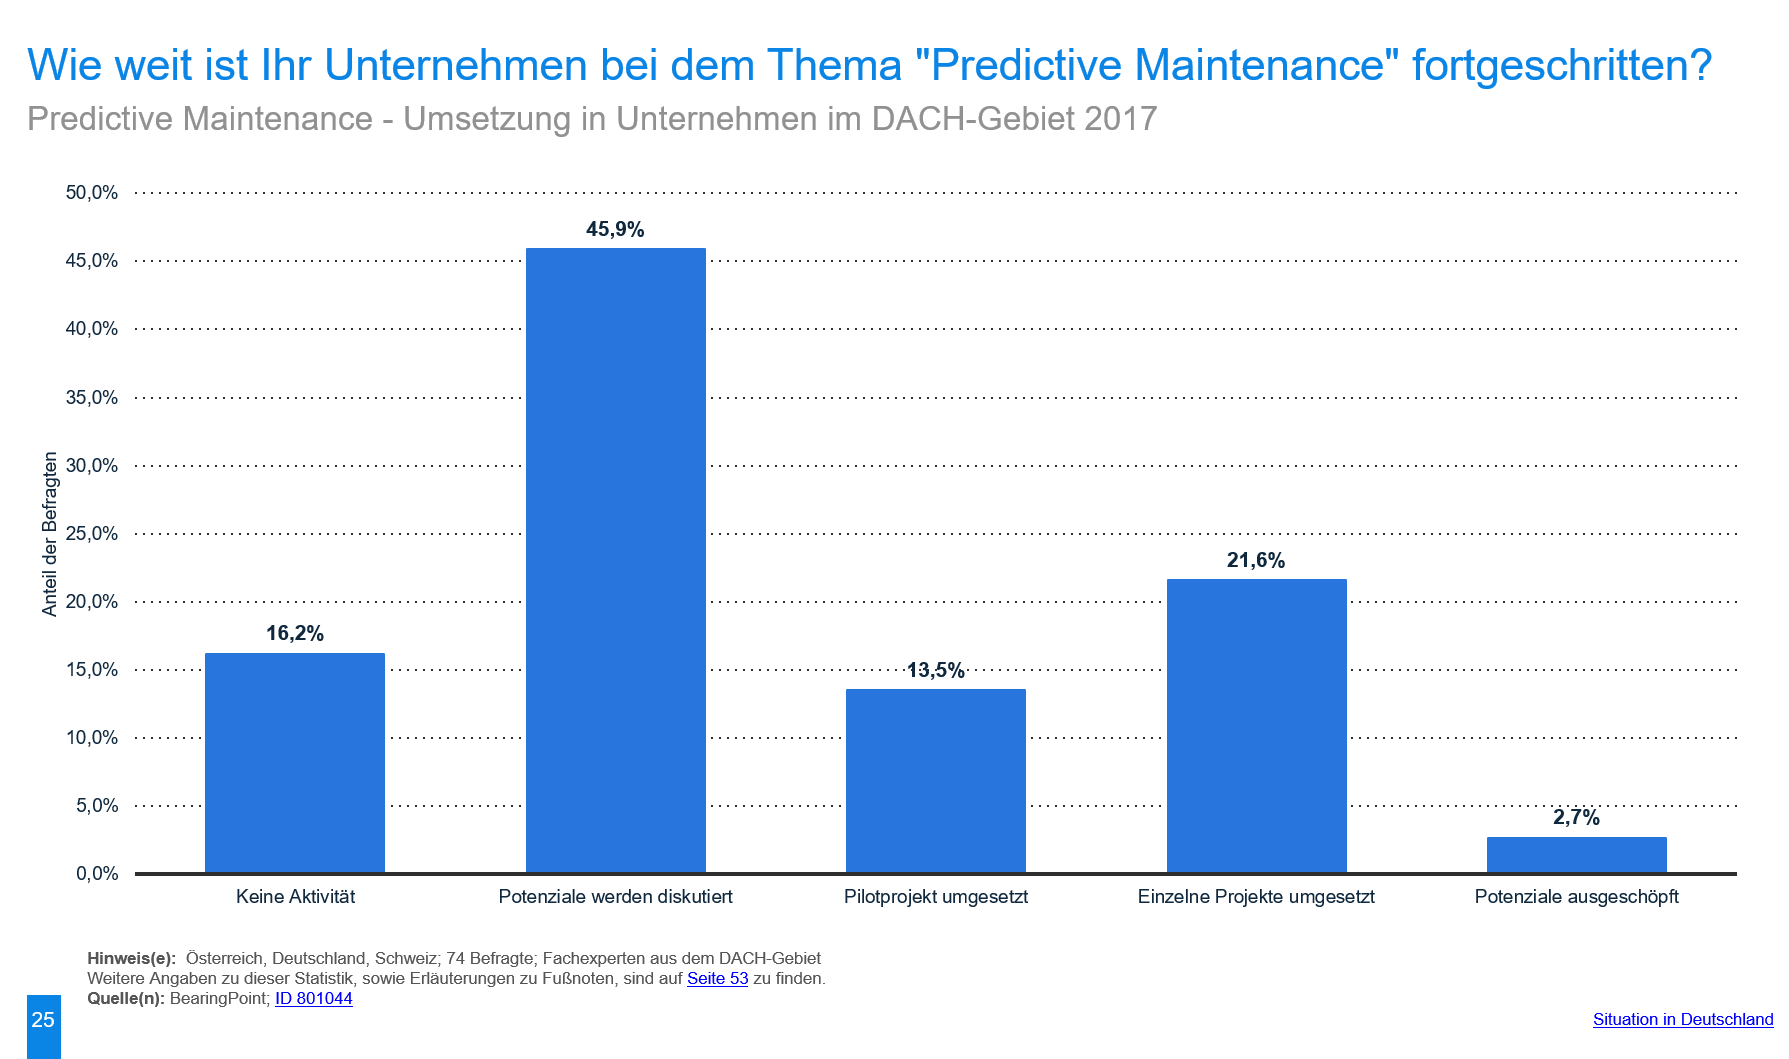
\includegraphics[scale=0.45]{picture/PM}
\caption{Predictive Maintenance in der Industrie (Chancen und Herausforderungen von Predictive Maintenance in der Industrie, Seite 25)}
\label{fig:Smart Factory - Genutzte Technologien in Deutschland 2017}
\end{figure}

\subsection{Künstliche Intelligenz für intelligente Sensoren}
Aber nicht nur im Bereich des PdM ist die Kombination selbst-lernender Systeme mit smart Sensoren effektiv. Da smarte Sensoren oft als WSN agieren stellt die Kommunikation untereinander einen große Herausforderung dar. Aktuelle Forschung beschäftigt sich damit wie mithilfe Künstlicher Neuronaler Netzwerke der Kommunikationsaufwand zwischen Sensoren verringert werden kann indem eine Datenvorverarbeitung schon im Lokalen System stattfindet. Dabei ist die größte Herausforderung die Neuronalen Netzwerke so zu Optimieren dass sie nicht die Vorteile ihres Einsatzes durch erhöhten Leistungsbedarf revidieren. Vor allem auf den Stromverbrauch muss dabei geachtet werden um die Einsatzdauer der Wireless Sensors wenn möglich zu erhöhen und nicht zu verringern.

\cite[Seite 3 ff.]{Talaska.2018}   
\newpage
\subsection{Zukunft und Herausforderungen}
%post SPS, Vernetzungsprobleme
Dieses Kommunikationsproblem wird noch verschärft durch das so genannte ''K-coverage problem''. Um eine zuverlässige und möglichst langfristige Abdeckung eines Bereiches mit Sensoren zu erreichen werden redundante Sensoren mit teilweise überlappenden Erkennungsbereichen benötigt. Damit stellt sich die Frage, wie viele Geräte werden mindestens benötigt um einen bestimmten Bereich zu überwachen. Es werden in Zukunft leistungsfähige Optimierungsalgorithmen benötigt werden um skalierbar zu bleiben. 
Wenn diese Hürden überwunden werden kann, kann sich der Sensor- und Automatisierungsmarkt immer weiter vom Einsatz speicherprogrammierbarer Steuerungen entfernen. Damit können intelligente und vernetzte Sensoren mit ihrer Modularität und Geschwindigkeit die Automatisierungsanforderungen der Zukunft bewältigen.

\cite[Seite 3 ff.]{Elhoseny.2019}  
\newpage

\section{Schlusswort}
Intelligente Sensoren sind nach Recherchen erkennbar unabdingbar für die heutige Zeit als auch für die Zukunft der Industrie. Im Moment ist man dabei diese Sensoren flächendeckend für Industrie 4.0 zu integrieren. Zahlreiche Beispiele befinden sich in der Logistik und Produktion, als auch spezifisch in der Landwirtschaft oder in der Automobilindustrie. Trotz dessen das wir in der 4. Generation der industriellen Revolution sind sieht man, dass das Thema noch viel Spielraum nach oben hat. Die intelligenten Sensoren sind die Grundbausteine um die Ziele der digitalen Zukunft umzusetzen. Sie werden über kurz oder lang nicht nur in der Industrie, sondern überall im Alltag in verschiedenen Bereichen vertreten sein. Wie in jeder Revolution werden auch die intelligenten Sensoren in naher Zukunft nicht mehr wegzudenken sein. Wir können uns auf eine SMARTe Zukunft freuen.

\newpage



\newpage
\section{Eidesstattliche erklärung}
Hiermit erkläre wir, dass wir die vorliegende Wissenschaftliche Arbeit selbständig verfasst und keine anderen als die angegebenen Hilfsmittel benutzt haben.
Die Stellen der Wissenschaftliche Arbeit, die anderen Quellen im Wortlaut oder dem Sinn nach entnommen wurden, sind durch Angaben der Herkunft kenntlich gemacht. Dies gilt auch für Zeichnungen, Skizzen, bildliche Darstellungen sowie für Quellen aus dem Internet.
\clearpage
\listoffigures
\newpage
\bibliographystyle{plain}
\bibliography{LiteraturIntelligenteSensoren}


\end{document}